\documentclass[oneside,fleqn,11pt]{book}
\usepackage[a4paper, total={7.2in, 10.3in}]{geometry}
\usepackage{tikz}
\usetikzlibrary{calc}
\usepackage{setspace}
\usepackage{graphicx}
\usepackage{amsmath}
\usepackage{amssymb}
\DeclareMathOperator\dx{\mathrm{d}\mathit{x}}
\DeclareMathOperator\cis{cis}
\DeclareMathOperator\sech{sech}
\DeclareMathOperator\csch{csch}
\DeclareMathOperator\arsinh{arsinh}
\DeclareMathOperator\arcosh{arcosh}
\DeclareMathOperator\artanh{artanh}
\DeclareMathOperator\Nset{\mathbb{N}}
\DeclareMathOperator\Zset{\mathbb{Z}}
\DeclareMathOperator\Qset{\mathbb{Q}}
\DeclareMathOperator\Rset{\mathbb{R}}
\DeclareMathOperator\Iset{\mathbb{I}}
\DeclareMathOperator\Cset{\mathbb{C}}

\usepackage{pgfplots}
\graphicspath{ {./images/} }
\usepackage{bookmark}
\setcounter{tocdepth}{0}
\usepackage{import}
\usepackage{mathtools}

\makeatletter
\g@addto@macro\bfseries{\boldmath}
\makeatother

\DeclarePairedDelimiter{\ceil}{\lceil}{\rceil}
\hypersetup{
	colorlinks   = true, %Colours links instead of ugly boxes
	urlcolor     = blue, %Colour for external hyperlinks
	linkcolor    = black, %Colour of internal links
	citecolor   = red %Colour of citations
}

\newcommand{\tikzAngleOfLine}{\tikz@AngleOfLine}
\def\tikz@AngleOfLine(#1)(#2)#3{%
	\pgfmathanglebetweenpoints{%
		\pgfpointanchor{#1}{center}}{%
		\pgfpointanchor{#2}{center}}
	\pgfmathsetmacro{#3}{\pgfmathresult}%
}

% math font
\usepackage{amsmath}
\usepackage{amssymb}
\usepackage{amsthm}
\usepackage{mathtools}
%\usepackage{arev}

% color
\usepackage[table]{xcolor}

\usepackage[many]{tcolorbox}
\usepackage{pifont}
\usepackage{hyperref}
\usepackage{blindtext}
\counterwithin*{chapter}{part}
\newcommand*{\Part}[2][\partheading]{%
  \refstepcounter{part}%
  \def\partheading{#2}%
  \part*{#2}%
  \addcontentsline{toc}{part}{#1}%
}
% \hypersetup{%
% 	linktoc=all,%
% 	bookmarksnumbered,%
% 	bookmarksopen,%
% 	hidelinks}
% \usepackage{bookmark}
% \bookmarksetup{
% 	addtohook={%
% 		\ifnum\bookmarkget{level}=0%
% 		\bookmarksetup{color=red}%
% 		\fi%
% 		\ifnum\bookmarkget{level}=1%
% 		\bookmarksetup{color=blue}%
% 		\fi%
% 		\ifnum\bookmarkget{level}=2%
% 		\bookmarksetup{color=teal}%
% 		\fi}}
% % enumerate
\usepackage[inline]{enumitem}
\usepackage{multicol}
\usepackage[inline]{enumitem}
\usepackage{tasks}
\usepackage{caption}
\usepackage{subcaption}
\usepackage{cancel}

\renewcommand\rmdefault{ptm}
\renewcommand\sfdefault{ptm}

\tcbset{
	colframe=magenta,
	colback=magenta!12!white,
	boxed title style={colback=magenta},
	breakable,
	enhanced,
	sharp corners,
	boxsep=1pt,
	attach boxed title to top left={yshift=-\tcboxedtitleheight,  yshifttext=-.75\baselineskip},
	boxed title style={boxsep=1pt,sharp corners},
	fonttitle=\bfseries\sffamily,
	drop lifted shadow
}
\newtcolorbox{solution}[1][]{
	no shadow,
	top=2ex,
	boxrule=0pt,
	leftrule=1.4pt,
	title={Solution},
	colframe=green!79!blue,
	colback=green!12!white,
	boxed title style={colback=green!79!blue},
	overlay unbroken and first={
		\node[below right,font=\small,color=magenta,text width=.8\linewidth]
		at (title.north east) {#1};
	}
}
\newtcolorbox[auto counter,number within=chapter,number format=\arabic]{activity}[1][]{
	title={Activity~\thetcbcounter},
	colframe=green,
	colback=green!22!white,
	coltitle=black,
	boxed title style={colback=green},
	overlay unbroken and first={
		\node[below right,font=\small,color=green,text width=.8\linewidth]
		at (title.north east) {#1};
	}
}
\newtcolorbox[auto counter,number within=chapter,number format=\arabic]{definition}[1][]{
	title={Definition~\thetcbcounter},
	colframe=blue,
	colback=blue!12!white,
	boxed title style={colback=blue},
	overlay unbroken and first={
		\node[below right,font=\small,color=blue,text width=.8\linewidth]
		at (title.north east) {#1};
	}
}
\newtcolorbox[auto counter,number within=chapter,number format=\arabic]{theorem}[1][]{
	title={Theorem~\thetcbcounter},
	colframe=violet,
	colback=violet!12!white,
	fontupper=\itshape,
	boxed title style={colback=violet},
	overlay unbroken and first={
		\node[below right,font=\small,color=violet,text width=.8\linewidth]
		at (title.north east) {#1};
	}
}
\newtcolorbox[auto counter,number within=chapter,number format=\arabic]{example}[1][]{
	title={Example~\thetcbcounter},
	colframe=magenta,
	colback=magenta!12!white,
	boxed title style={colback=magenta},
	overlay unbroken and first={
		\node[below right,font=\small,color=magenta,text width=.8\linewidth]
		at (title.north east) {#1};
	}
}
\newtcolorbox[auto counter,number within=chapter,number format=\arabic]{exercise}[1][]{
	title={Exercise~\thetcbcounter},
	colframe=red,
	colback=red!12!white,
	boxed title style={colback=red},
	overlay unbroken and first={
		\node[below right,font=\small,color=red,text width=.8\linewidth]
		at (title.north east) {#1};
	}
}
\newtcolorbox[auto counter,number within=chapter,number format=\arabic]{generality}[1][]{
	title={Generality~\thetcbcounter},
	colframe=teal,
	colback=teal!12!white,
	boxed title style={colback=teal},
	overlay unbroken and first={
		\node[below right,font=\small,color=teal,text width=.8\linewidth]
		at (title.north east) {#1};
	}
}
\newtcolorbox[auto counter,number within=chapter,number format=\arabic]{property}[1][]{
	title={Property~\thetcbcounter},
	colframe=teal,
	colback=teal!12!white,
	boxed title style={colback=teal},
	overlay unbroken and first={
		\node[below right,font=\small,color=teal,text width=.8\linewidth]
		at (title.north east) {#1};
	}
}
\newtcolorbox{remark}[1][]{
	title={\scalebox{1.75}{\raisebox{-.25ex}{\ding{43}}}~Remark},
	colframe=yellow!45!white,
	colback=yellow!45!white,
	coltitle=violet,
	fontupper=\sffamily,
	boxed title style={colback=yellow!45!white},
	boxed title style={boxsep=1ex,sharp corners},%%
	overlay unbroken and first={
		\node[below right,font=\normalsize,color=red,text width=.8\linewidth]
		at (title.north east) {#1};
	}
}
\newtcolorbox{note}[1][]{
	title={\scalebox{1.75}{\raisebox{-0.25ex}{\ding{45}}}~Note},
	colframe=yellow!45!white,
	colback=yellow!45!white,
	coltitle=violet,
	fonttitle=\bfseries\sffamily,
	fontupper=\sffamily,
	boxed title style={colback=yellow!45!white},
	boxed title style={boxsep=1ex,sharp corners},%%
	overlay unbroken and first={
		\node[below right,font=\normalsize,color=red,text width=.8\linewidth]
		at (title.north east) {#1};
	}
}

\makeatletter
\g@addto@macro\bfseries{\boldmath}
\makeatother

\title{Further Mathematics Notes - Core Pure}
\author{Xingzhi Lu}
\date{}

\begin{document}
\everymath{\displaystyle}
\maketitle
\tableofcontents
\pagebreak
\chapter{Complex numbers}
\section{Cartesian form for expressing complex numbers}
\begin{tikzpicture}
    \draw[->, thick] (-0.5,0)--(4,0) node[right]{$x$};
    \draw[->, thick] (0,-0.5)--(0,3.5) node[above]{$y$};
    \coordinate (O) at (0,0);
    \coordinate (A) at (3.5,0);
    \coordinate (B) at (3.5,3);
    \draw [dotted] (A) -- (B);
    \draw [->] (O) -- (B);
    \node[below] at (2,0) {a};
    \node [right] at (3.5,1.5) {b};
    \node [above left] at (1.75, 1.5) {r};
    \tikzAngleOfLine(O)(A){\AngleStart}
    \tikzAngleOfLine(O)(B){\AngleEnd}
    \draw[black,<->] (O)+(\AngleStart:0.7cm) arc (\AngleStart:\AngleEnd:0.7cm);
    \node [above right] at (0.65, 0) {$\theta$};
\end{tikzpicture}
\begin{itemize}
    \item $z=a+bi$
    \item $\operatorname{Re}(z) = a$, $\operatorname{Im}(z) = b$
    \item $|z|=\sqrt{a^2+b^2}$
\end{itemize}

\section{Multiplying complex numbers}
\begin{itemize}
    \item $i^2 = -1$
    \item Multiply out the terms as if they are polynomials
\end{itemize}

\section{Conjugation of complex numbers}
\begin{itemize}
    \item $|z|=|z^*|$
    \item $z\cdot z^*= |z|^2$
    \item If $z=z*$ then $z$ is a real number
    \item If $z=-z*$ then $z$ is a pure imaginary number
\end{itemize}
\subsection{Roots of quadratic equations}
If $a+bi$ is the root of a quadratic equation, then $a-bi$ is also a root of the same quadratic equation.
\chapter{Argand diagrams}
\section{Modulus and argument}
For $z=x+yi$:
\begin{description}
    \item[Modulus] $|z| = \sqrt{x^2+y^2}$
    \item[Argument] $\theta = \arg z = \arctan\left(\frac{y}{x}\right)$
\end{description}

\subsection{Modulus-argument form}
For complex number $z$ with $|z|=r$ and $\arg z = \theta$:
$$z=r\left(\cos\theta + i\sin\theta\right)=r\cis\theta$$

\subsection{Calculations with arguments}
\begin{itemize}
    \item $\arg\left(z_1z_2\right)=\arg z_1 +\arg z_2$
    \item $\arg\left(\frac{z_1}{z_2}\right)=\arg z_1-\arg z_2$
\end{itemize}

\subsection{Calculations with modulus}
\begin{itemize}
    \item $|z_1z_2|=|z_1||z_2|$
    \item $\left|\dfrac{z_1}{z_2}\right|=\dfrac{|z_1|}{|z_2|}$
    \item $\left||z_1|-|z_2|\right| \leq |z_1 \pm z_2| \leq |z_1|+|z_2|$ (same as triangular inequalities)
\end{itemize}

\section{Loci of different expressions}
\subsection{Circle}
\begin{itemize}
    \item $|z| = a$: circle with centre $O$, radius $a$
    \item $|z-z_0|=a$: circle with centre $z_0$, radius $a$
    \item $|z-z_0|<a$: circle with centre $z_0$, radius $a$, shaded in
    \item $|z-z_0|>a$: circle with centre $z_0$, radius $a$, outside of circle shaded
\end{itemize}
\subsection{Perpendicular bisector}
\begin{itemize}
    \item $|z-z_1|=|z-z_2|$: $z$ on perpendicular bisector of $z_1z_2$
    \item $|z-z_1|<|z-z_2|$ / $|z-z_1|>|z-z_2|$: on the left / right side of perpendicular bisector, bisector = dotted line
\end{itemize}
\subsection{Argument angle}
\begin{itemize}
    \item $\arg z = \theta$: ray starting from origin, angle with x-axis = $\theta$
    \item $\arg (z-z_0) = \theta$: ray starting from $z_0$, angle with horizontal = $\theta$
\end{itemize}
\subsection{Ellipse}
\begin{itemize}
    \item $|z-z_1|+|z-z_2|=2a$: ellipse with focus at $z_1$ and $z_2$, longest diameter = $2a$
\end{itemize}


\chapter{Series}
\section{Summation of squares}
$$\sum_{r=1}^{n} r^2=\dfrac{n(n+1)(2n+1)}{6}$$
\subsection{Proof (without mathematical induction)}


\section{Summation of cubes}
$$\sum_{r=1}^{n} r^3=\dfrac{(n(n+1))^2}{4}$$
\subsection{Proof (without mathematical induction)}
\chapter{Roots of polynomials}
\section{Vieta's Law}
For $a_{n}x^{n}+a_{n-1}x^{n-1}+\cdots +a_{1}x+a_{0}=0$:
\begin{itemize}
    \item $\sum x_i=-\dfrac{a_{n-1}}{a_n}$
    \item $\sum x_ix_j=\dfrac{a_{n-2}}{a_n}$
    \item $\sum x_ix_jx_k = -\dfrac{a_{n-3}}{a_n}$
    \item $\sum _{1\leq i_{1}<i_{2}<\cdots <i_{k}\leq n}\left(\prod _{j=1}^{k}r_{i_{j}}\right)=(-1)^{k}{\frac {a_{n-k}}{a_{n}}}$
    \item $\prod x_i=(-1)^n\dfrac{a_0}{a_n}$
\end{itemize}
\chapter{Volumes of revolution}
\section{Finding volumes of revolution}
Volume = $\pi\int y^2 \: dx$ or $\pi\int x^2 \: dy$
\chapter{Matrices}
\section{Basic calculations}
\subsection{Addition / subtraction}
$(\mathbf {A}+\mathbf {B})_{i,j}=\mathbf {A}_{i,j}+{\mathbf {B}}_{i,j},\quad 1\leq i\leq m,\quad 1\leq j\leq n$\\
$(\mathbf {A}-\mathbf {B})_{i,j}=\mathbf {A}_{i,j}-{\mathbf {B}}_{i,j},\quad 1\leq i\leq m,\quad 1\leq j\leq n$
\subsection{Scalar multiplication}
$(c\mathbf{A})_{i,j}=c\cdot A_{i,j}$
\subsection{Matrix multiplication}
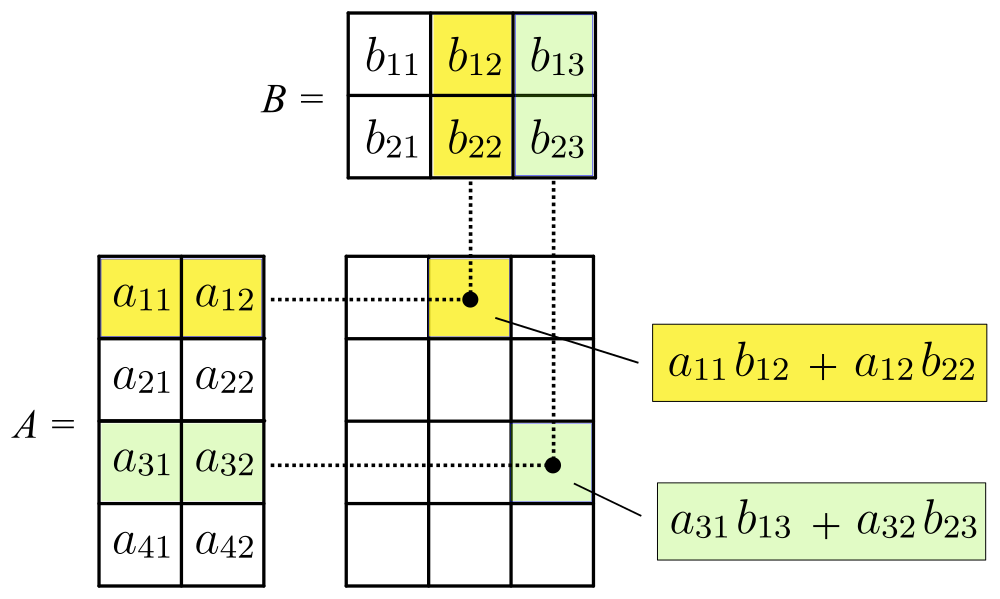
\includegraphics[width=0.35\textwidth]{MatrixMultiplication}

\subsection{Transposition}
$(\mathbf{A}^\mathrm{T})_{i,j}=A_{j,i}$

\section{Special matrices}
\begin{description}
    \item[Square matrix:] The number of rows and columns are the same
    \item[Zero matrix:] All of the elements are zero
    \item[Identity matrix:] A square matrix in which all the elements on the leading diagonal are 1 and the remaining elements are 0, denoted by $\mathbf{I}_k$ for $k\times k$ identity matrix
\end{description}


\section{Determinants}

\subsection{$2\times2$ matrices}
$\begin{vmatrix}a&b\\c&d\end{vmatrix}=ad-bc$

\subsection{$3\times3$ matrices}

$\begin{vmatrix}a&b&c\\d&e&f\\g&h&i\end{vmatrix}=a\begin{vmatrix}e&f\\h&i\end{vmatrix}-b\begin{vmatrix}d&f\\g&i\end{vmatrix}+c\begin{vmatrix}d&e\\g&h\end{vmatrix}=aei+bfg+cdh-ceg-bdi-afh$

\subsection{Singular matrices}
\begin{itemize}
    \item Singular matrices are square matrices with a determinant of 0
    \item It does not have an inverse
    \item If $\mathbf{A}$ and $\mathbf{B}$ are non-singular matrices, then $(\mathbf{AB})^{-1}=\mathbf{B}^{-1}\mathbf{A}^{-1}$
\end{itemize}



\subsection{Properties of determinants}
\begin{itemize}
    \item $\det(\mathbf{AB})=\det(\mathbf{A})\det(\mathbf{B})=\det(\mathbf{B})\det(\mathbf{A})=\det(\mathbf{BA})$
    \item $\det(k\mathbf{A})=k^n\det(\mathbf{A})$ ($\mathbf{A}$ is a $n\times n$ matrix)
\end{itemize}


\section{Inverse matrices}
\subsection{$2\times2$ matrices}
$\begin{bmatrix}
        a & b \\c & d
    \end{bmatrix}^{-1}=\dfrac{1}{ad-bc}\begin{bmatrix}
        d & -b \\-c & a
    \end{bmatrix}$

\subsection{$3\times3$ matrices}
$\mathbf {A} ^{-1}={\begin{bmatrix}a&b&c\\d&e&f\\g&h&i\\\end{bmatrix}}^{-1}={\frac {1}{\det(\mathbf {A} )}}{\begin{bmatrix}\,A&\,B&\,C\\\,D&\,E&\,F\\\,G&\,H&\,I\\\end{bmatrix}}^{\mathrm {T} }={\frac {1}{\det(\mathbf {A} )}}{\begin{bmatrix}\,A&\,D&\,G\\\,B&\,E&\,H\\\,C&\,F&\,I\\\end{bmatrix}}$\\
$\begin{alignedat}{6}A&={}&(ei-fh),&\quad &D&={}&-(bi-ch),&\quad &G&={}&(bf-ce),\\B&={}&-(di-fg),&\quad &E&={}&(ai-cg),&\quad &H&={}&-(af-cd),\\C&={}&(dh-eg),&\quad &F&={}&-(ah-bg),&\quad &I&={}&(ae-bd).\\\end{alignedat}$

\subsection{Solving equations with matrices}
If $\mathbf{A}\begin{pmatrix}
        x \\y\\z
    \end{pmatrix}=\mathbf{v}$ then $\begin{pmatrix}
        x \\y\\z
    \end{pmatrix}=\mathbf{A}^{-1}\mathbf{v}$
\begin{description}
    \item[Consistent system of linear equations:] there is at least one set of values that satisfies all the equations simultaneously
    \item[Inconsistent:] such set of values does not exist
\end{description}

\subsection{Possible outcomes of solutions}
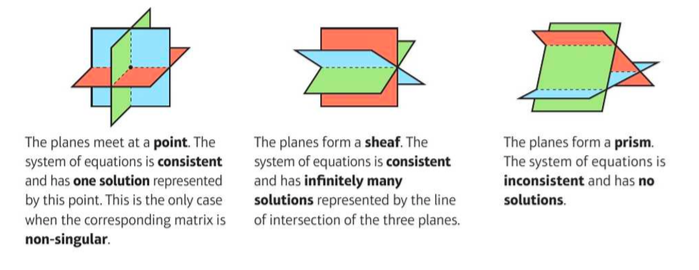
\includegraphics[width=0.75\textwidth]{equations}\\
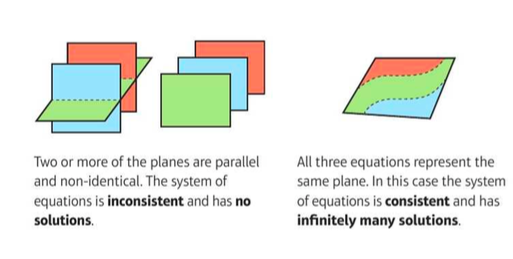
\includegraphics[width=0.5\textwidth]{equations2}
\chapter{Linear transformations}
\section{Linear transformations in 2D}
\subsection{Properties}
If $L(\vec{v})$ is linear:
\begin{enumerate}
    \item $L(\vec{v})$ should always map the origin onto itself
    \item $L(\vec{v})$ can be represented by a matrix
    \item $L(\vec{v_1}+\vec{v_2})=L(\vec{v_1})+L(\vec{v_2})$ (closure in addition)
    \item $L(\lambda\vec{v_1})=\lambda L(\vec{v_1})$ (closure in scalar multiplication)
\end{enumerate}
\subsection{Invariant points and lines}
\begin{description}
    \item[Invariant points:] Points which are mapped onto themselves under the given transformation
    \item[Invariant lines:] Lines which map onto themselves
\end{description}

\subsection{Reflection}
\begin{description}
    \item[Reflection in $y$-axis:] $\begin{pmatrix}
                  -1 & 0 \\0&1
              \end{pmatrix}$, invariant points: points on the $y$-axis; invariant lines: $x=0$, $y=k$
    \item[Reflection in $x$-axis:] $\begin{pmatrix}
                  1 & 0 \\0&-1
              \end{pmatrix}$, invariant points: points on the $x$-axis; invariant lines: $y=0$, $x=k$
    \item[Reflection in line $y=x$:] $\begin{pmatrix}
                  0 & 1 \\1&0
              \end{pmatrix}$, invariant points: points on $y=x$; invariant lines: $y=x$, $y=-x+k$
    \item[Reflection in line $y=-x$:] $\begin{pmatrix}
                  0 & -1 \\-1&0
              \end{pmatrix}$, invariant points: points on $y=-x$; invariant lines: $y=-x$, $y=x+k$
\end{description}

\subsection{Rotation}
\begin{description}
    \item[Rotation through angle $\theta$ anticlockwise about the origin] $\begin{pmatrix}
                  \cos\theta & -\sin\theta \\\sin\theta&\cos\theta
              \end{pmatrix}$
    \item[Invariant points:] Only $(0,0)$
    \item[Invariant lines:] When $\theta=180\textdegree$ any line passing through the origin is an invariant line, otherwise no invariant lines
\end{description}

\subsection{Enlargement / stretches}
\begin{description}
    \item[Transformation matrix] $\begin{pmatrix}
                  a & 0 \\ 0 & b
              \end{pmatrix}$ = a stretch of scale factor $a$ parallel to the $x$-axis and scale factor $b$ parallel to the $y$-axis
    \item[Invariant lines] $x$- and $y$-axes for all stretches
          \begin{itemize}
              \item Stretch parallel to the $x$-axes: any line parallel to the $x$-axes
              \item Stretch parallel to the $y$-axes: any line parallel to the $y$-axes
          \end{itemize}
    \item[Invariant points] The origin is always an invariant point
          \begin{itemize}
              \item Stretch parallel to the $x$-axes: points on the $y$-axes
              \item Stretch parallel to the $y$-axes: points on the $x$-axes
          \end{itemize}
    \item[Change in area] $\det(\mathbf{M}) = \text{area scale factor}$
\end{description}

\section{Linear transformations in 3D}
\begin{description}
    \item[Reflection in plane $x=0$] $\begin{pmatrix}
                  -1 & 0 & 0 \\
                  0  & 1 & 0 \\
                  0  & 0 & 1
              \end{pmatrix}$
    \item[Reflection in plane $y=0$] $\begin{pmatrix}
                  1 & 0  & 0 \\
                  0 & -1 & 0 \\
                  0 & 0  & 1
              \end{pmatrix}$
    \item[Reflection in plane $z=0$] $\begin{pmatrix}
                  1 & 0 & 0  \\
                  0 & 1 & 0  \\
                  0 & 0 & -1
              \end{pmatrix}$
    \item[Rotation angle $\theta$ anticlockwise about the $x$-axis] $\begin{pmatrix}
                  1 & 0          & 0           \\
                  0 & \cos\theta & -\sin\theta \\
                  0 & \sin\theta & \cos\theta
              \end{pmatrix}$
    \item[Rotation angle $\theta$ anticlockwise about the $y$-axis] $\begin{pmatrix}
                  \cos\theta  & 0 & \sin\theta \\
                  0           & 1 & 0          \\
                  -\sin\theta & 0 & \cos\theta
              \end{pmatrix}$
    \item[Rotation angle $\theta$ anticlockwise about the $z$-axis] $\begin{pmatrix}
                  \cos\theta & -\sin\theta & 0 \\
                  \sin\theta & \cos\theta  & 0 \\
                  0          & 0           & 1
              \end{pmatrix}$
\end{description}





\chapter{Proof by induction}
\section{Proof by mathematical induction}
\begin{enumerate}
    \item Prove the general statement is true for $n=0$ / $n=1$ / the smallest possible value of $n$
    \item Assume the general statement is true for $n=k$
    \item Show that the general statement is true for $n=k+1$
    \item The general statement is then true for all positive integers $n$
\end{enumerate}
\chapter{Vectors}
\section{Expressing linear equations}
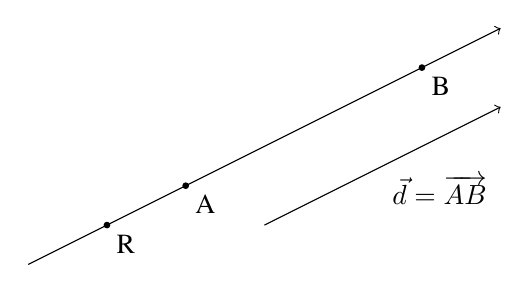
\begin{tikzpicture}
    \draw[->] (0,0) -- (6,3);
    \node[below right] at (1,0.5) {R};
    \filldraw [black] (1,0.5) circle (1pt);
    \node[below right] at (2,1) {A};
    \filldraw [black] (2,1) circle (1pt);
    \node[below right] at (5,2.5) {B};
    \filldraw [black] (5,2.5) circle (1pt);
    \draw[->] (3,0.5) -- (6,2);
    \node[below right] at (4.5,1.25) {$\vec{d}=\overrightarrow{AB}$};
\end{tikzpicture}

\subsection{Vector form}
$\vec{r}=\vec{a}+t\vec{d}$ or $(\vec{r}-\vec{a})\times\vec{d}=0$ / $(\vec{r}-\vec{a})\times\vec{b}=0$
\subsection{Parametric form}
$\begin{cases}
        x=x_0+tu \\
        y=y_0+tv \\
        z=z_0+tw
    \end{cases}$
\subsection{Cartesian form}
$\dfrac{x-x_0}{u}=\dfrac{y-y_0}{v}=\dfrac{z-z_0}{w}(=t)$

\section{Expressing planes}
\subsection{Vector form}
$\vec{r} \cdot \vec{n} = \vec{r} \cdot \vec{a}$ ($\vec{n}$ = normal, $\vec{a}$ = a point on plane)
\subsection{Parametric form}
$\vec{r}=\vec{a}+\lambda\vec{b}+\mu\vec{c}$
\subsection{Cartesian form}
When $\vec{n} = \begin{pmatrix}a\\b\\c\end{pmatrix}$: $ax+by+cz=d$

\section{Formulae}
\subsection{Dot and cross product}

\begin{itemize}
    \item $\vec{a} \cdot \vec{b} = |\vec{a}||\vec{b}|\cos\theta=x_1x_2+y_1y_2+z_1z_2$
          \begin{description}
              \item $\vec{a}\perp\vec{b}$: $\vec{a} \cdot \vec{b} = 0$
              \item $\cos\theta = \dfrac{\vec{a} \cdot \vec{b}}{|\vec{a}||\vec{b}|}$
          \end{description}
    \item $\vec{a} \times \vec{b} = \begin{pmatrix} x_1 \\ x_2 \\ x_3\end{pmatrix} \times \begin{pmatrix} y_1 \\ y_2 \\ y_3\end{pmatrix}=\begin{pmatrix} x_2y_3-x_3y_2 \\ x_3y_1-x_1y_3 \\ x_1y_2-x_2y_1\end{pmatrix}$
          \begin{description}
              \item[Calculating cross product using matrix:] $\begin{vmatrix}
                            \vec{i} & \vec{j} & \vec{k} \\
                            x_1     & x_2     & x_3     \\
                            y_1     & y_2     & y_3
                        \end{vmatrix}$
              \item $\vec{a} \times \vec{b} \perp \vec{a}$ and $\vec{a} \times \vec{b} \perp \vec{n}$, so $\vec{a} \times \vec{b} = \vec{n}$
              \item $|\vec{a} \times \vec{b}| = |\vec{a}||\vec{b}|\sin\theta$
              \item $\vec{a}\parallel\vec{b}$: $\vec{a}=\lambda\vec{b}$; $\vec{a} \times \vec{b} = \vec{0}$

          \end{description}
\end{itemize}

\section{Questions}
\subsection{Angle between planes}
\begin{enumerate}
    \item Find the normal of the two planes
    \item Use $\theta = \cos^{-1}\dfrac{\vec{n_1}\cdot\vec{n_2}}{|\vec{n_1}||\vec{n_2}|}$ to find the angle between planes
    \item If $\theta>90$ than the angle is $180-\theta$
\end{enumerate}
\subsection{Angle between plane and line}
$\phi = 90-\cos^{-1}\dfrac{\vec{n}\cdot\vec{d}}{|\vec{n}||\vec{d}|}$ or $\phi =\sin^{-1}\dfrac{\vec{n}\cdot\vec{d}}{|\vec{n}||\vec{d}|}$
\subsection{Finding distances between point and line}
%\begin{tikzpicture}
%	\coordinate (P) at (4,2);
%	\coordinate (T) at (2,1);
%	\coordinate (N) at (0.5,4);
%	\draw[<-] (0,0) -- (5,2.5);
%	\node[below right] at (4,2) {P};
%	\filldraw [black] (4,2) circle (1pt);
%	\node[below right] at (2,1) {T};
%	\draw [dotted] (2,1) -- (0.5, 4);
%	\draw [->] (4,2) -- (0.5,4);
%	\node[left] at (0.5,4) {N};
%	\tikzAngleOfLine(P)(T){\AngleStart}
%	\tikzAngleOfLine(P)(N){\AngleEnd}
%	\draw[black,<->] (P)+(\AngleStart:0.7cm) arc (\AngleStart:\AngleEnd:0.7cm);
%	\node[left] at (3.7,2.05) {$\theta$};
%\end{tikzpicture}\\
%Distance of $N$ to $\overrightarrow{PT}$:
%$|\overrightarrow{PT}| = |\overrightarrow{PN}|\cos \theta = \dfrac{\overrightarrow{PN}\cdot\vec{d}}{|\vec{d}|}$\\ $|\vec{d}|=\sqrt{|\overrightarrow{PN}|^2-|\overrightarrow{PT}|^2}=\dfrac{|(N-P)\times(P-N)|}{|P-T|}=\dfrac{|(T-P)\times(P-N)|}{|P-T|}$
For point $\textbf{x}_0$ to line $\textbf{x}_1\textbf{x}_2$: $d=\dfrac{|(\textbf{x}_2-\textbf{x}_1)\times(\textbf{x}_1-\textbf{x}_0)|}{|\textbf{x}_2-\textbf{x}_1|}=\dfrac{|(\textbf{x}_0-\textbf{x}_1)\times(\textbf{x}_0-\textbf{x}_2)|}{|\textbf{x}_2-\textbf{x}_1|}$





\subsection{Finding distances from point to plane}
When $P=(x_0,y_0,z_0)$ and the plane has equation $ax+by+cz-d=0$:
\begin{math}\text{distance}=\dfrac{|ax_0+by_0+cz_0+d|}{\sqrt{a^2+b^2+c^2}}\end{math}
\subsection{Finding distances between lines}
$\text{distance}=\dfrac{|\overrightarrow{AB}\cdot\vec{n}|}{|\vec{n}|}$ ($\overrightarrow{AB}$ = any line that connects 2 lines together)
\subsection{Finding intersections between line and plane}
Write line in parametric form, substitute $x$, $y$ and $z$ into the equation for plane (Cartesian form)



\end{document}